\usetikzlibrary{arrows}
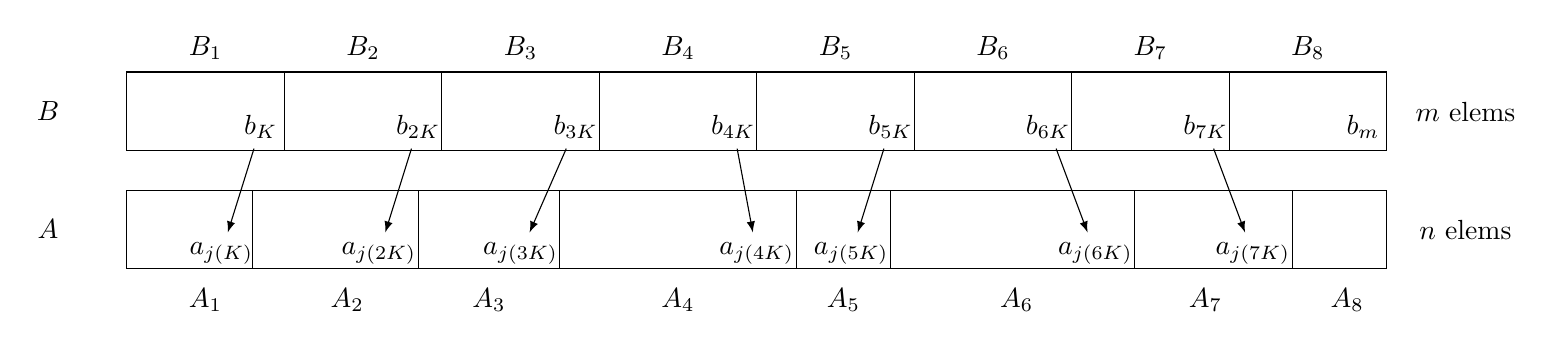
\begin{tikzpicture}

\draw (0,0) rectangle +(16,1);
\draw (0,1.5) rectangle +(16,1);

%\foreach \y in {0,2,4,6}
\foreach \x in {2,4,...,15} {
	\draw (\x,1.5) -- +(0,1);
}


\foreach \x in {1.6,3.7,5.5,8.5,9.7, 12.8, 14.8} {
	\draw (\x,0) -- +(0,1);
}

\node at (-1,2) {$B$};
\node at (-1,0.5) {$A$};

\node at (17, 2) {$m$ elems};
\node at (17,0.5) {$n$ elems};

%\node at (8,2) {$b_i < b_{i+1}$};
%\node at (8,0.5) {$a_i < a_{i+1}$};

\node (v1) at (1.7,1.8) {$b_K$};
\node (v3) at (3.7,1.8) {$b_{2K}$};
\node (v5) at (5.7,1.8) {$b_{3K}$};
\node (v7) at (7.7,1.8) {$b_{4K}$};
\node (v9) at (9.7,1.8) {$b_{5K}$};
\node (v11) at (11.7,1.8) {$b_{6K}$};
\node (v13) at (13.7,1.8) {$b_{7K}$};
\node at (15.7,1.8) {$b_{m}$};

\node (v2) at (1.2,0.2) {$a_{j(K)}$};
\node (v4) at (3.2,0.2) {$a_{j(2K)}$};
\node (v6) at (5,0.2) {$a_{j(3K)}$};
\node (v8) at (8,0.2) {$a_{j(4K)}$};
\node (v10) at (9.2,0.2) {$a_{j(5K)}$};
\node (v12) at (12.3,0.2) {$a_{j(6K)}$};
\node (v14) at (14.3,0.2) {$a_{j(7K)}$};

\node () at (1.0,2.8) {$B_1$};
\node () at (3.0,2.8) {$B_2$};
\node () at (5.0,2.8) {$B_3$};
\node () at (7.0,2.8) {$B_4$};
\node () at (9.0,2.8) {$B_5$};
\node () at (11.0,2.8) {$B_6$};
\node () at (13.0,2.8) {$B_7$};
\node () at (15.0,2.8) {$B_8$};

\node () at (1.0,-0.4) {$A_1$};
\node () at (2.8,-0.4) {$A_2$};
\node () at (4.6,-0.4) {$A_3$};
\node () at (7.0,-0.4) {$A_4$};
\node () at (9.1,-0.4) {$A_5$};
\node () at (11.3,-0.4) {$A_6$};
\node () at (13.7,-0.4) {$A_7$};
\node () at (15.5,-0.4) {$A_8$};

% \node at (7,3) {$K=\log m$};

\draw [-latex] (v1) edge (v2);
\draw [-latex] (v3) edge (v4);
\draw [-latex] (v5) edge (v6);
\draw [-latex] (v7) edge (v8);
\draw [-latex] (v9) edge (v10);
\draw [-latex] (v11) edge (v12);
\draw [-latex] (v13) edge (v14);
\end{tikzpicture}